\documentclass[12pt]{article}

\usepackage{sbc-template}
\usepackage[T1]{fontenc}
\usepackage[utf8]{inputenc}
\usepackage[brazilian]{babel}
\usepackage{graphicx,url}
\usepackage{array,booktabs}
\usepackage{amsmath,amssymb}
\usepackage{tikz}
\usetikzlibrary{arrows.meta,positioning}

\sloppy

\newcommand{\pend}[1]{\textbf{[PENDÊNCIA: #1]}}
% Arquivo gerado automaticamente por scripts/gerar_artefatos.py — NAO EDITAR A MAO
\newcommand{\nTotal}{29}
\newcommand{\nRevisadosPares}{23}
\newcommand{\pctRevisadosPares}{79,3\%}
\newcommand{\nPreprints}{6}
\newcommand{\pctPreprints}{20,7\%}
\newcommand{\nAplicaveisVaz}{27}
\newcommand{\nNaoAplicaveisVaz}{2}
\newcommand{\nImportados}{115}
\newcommand{\nDuplicados}{24}
\newcommand{\nTriados}{91}
\newcommand{\nRejeitados}{62}
\newcommand{\nAceitos}{29}
\newcommand{\nScholarDireto}{69}
\newcommand{\nScholarBalde}{84}
\newcommand{\nNatureExcl}{14}
\newcommand{\nNatureTotal}{77}
\newcommand{\nSnowballing}{15}
\newcommand{\nSementesSnowballing}{11}
\newcommand{\nStringsTotal}{17}
\newcommand{\nStringsIEEE}{7}
\newcommand{\nStringsPMC}{1}
\newcommand{\nStringsSD}{3}
\newcommand{\nStringsScopus}{6}
\newcommand{\nComumScholarNature}{63}
\newcommand{\nSoScholar}{6}
\newcommand{\nUniaoScholarNature}{83}
\newcommand{\nCamposTotalAud}{1102}
\newcommand{\nPontosRevisao}{138}
\newcommand{\nTriagemAceito}{22}
\newcommand{\nTriagemRessalvas}{5}
\newcommand{\nTriagemNaoConfiavel}{1}
\newcommand{\nTriagemIncerto}{1}
\newcommand{\nAnoDoisQuatro}{4}
\newcommand{\nAnoDoisCinco}{10}
\newcommand{\nAnoDoisSeis}{15}
\newcommand{\pctAnoDoisQuatro}{13,8\%}
\newcommand{\pctAnoDoisCinco}{34,5\%}
\newcommand{\pctAnoDoisSeis}{51,7\%}
\newcommand{\nPeriodicos}{11}
\newcommand{\pctPeriodicos}{37,9\%}
\newcommand{\nAnais}{12}
\newcommand{\pctAnais}{41,4\%}
\newcommand{\nPreArxiv}{3}
\newcommand{\nPreMedrxiv}{1}
\newcommand{\nPreRS}{1}
\newcommand{\nPreJMIR}{1}
\newcommand{\nContribNovoModelo}{17}
\newcommand{\pctContribNovoModelo}{58,6\%}
\newcommand{\nContribComparativo}{8}
\newcommand{\pctContribComparativo}{27,6\%}
\newcommand{\nContribEstatistica}{2}
\newcommand{\nContribPlataforma}{1}
\newcommand{\nContribOutro}{1}
\newcommand{\nPapelPrincipal}{25}
\newcommand{\pctPapelPrincipal}{86,2\%}
\newcommand{\nPapelSuplementar}{3}
\newcommand{\nPapelExtGen}{1}
\newcommand{\nMultiBase}{11}
\newcommand{\pctMultiBase}{37,9\%}
\newcommand{\nOutroPublico}{9}
\newcommand{\nPrivadoProprio}{5}
\newcommand{\nMultiBaseSobrep}{3}
\newcommand{\nModIMU}{27}
\newcommand{\pctModIMU}{93,1\%}
\newcommand{\nModPDNMS}{9}
\newcommand{\pctModPDNMS}{31,0\%}
\newcommand{\nModMetadados}{8}
\newcommand{\pctModMetadados}{27,6\%}
\newcommand{\nModSoPDNMS}{2}
\newcommand{\nTarTodas}{14}
\newcommand{\pctTarTodas}{48,3\%}
\newcommand{\nTarSubconj}{7}
\newcommand{\nTarNaoRep}{6}
\newcommand{\nTarNA}{2}
\newcommand{\nSensGiro}{25}
\newcommand{\nSensAcel}{24}
\newcommand{\nSensOutro}{1}
\newcommand{\nSensVazio}{3}
\newcommand{\nPunhoAmbos}{16}
\newcommand{\pctPunhoAmbos}{55,2\%}
\newcommand{\nPunhoNaoRep}{9}
\newcommand{\nPunhoDir}{1}
\newcommand{\nPunhoEsq}{1}
\newcommand{\nPunhoNA}{2}
\newcommand{\nPartRep}{21}
\newcommand{\pctPartRep}{72,4\%}
\newcommand{\nPartMin}{234}
\newcommand{\nPartMax}{469}
\newcommand{\nPartMediana}{469}
\newcommand{\nClasseRep}{22}
\newcommand{\nCenPDHC}{20}
\newcommand{\pctCenPDHC}{69,0\%}
\newcommand{\nCenPDDD}{15}
\newcommand{\pctCenPDDD}{51,7\%}
\newcommand{\nCenTresClasses}{7}
\newcommand{\pctCenTresClasses}{24,1\%}
\newcommand{\nCenDDHC}{2}
\newcommand{\nCenOutro}{5}
\newcommand{\nCenNA}{1}
\newcommand{\nRepBruta}{20}
\newcommand{\pctRepBruta}{69,0\%}
\newcommand{\nRepHandcrafted}{14}
\newcommand{\pctRepHandcrafted}{48,3\%}
\newcommand{\nRepTF}{4}
\newcommand{\nRepOutro}{4}
\newcommand{\nRepNA}{3}
\newcommand{\nFamDL}{22}
\newcommand{\pctFamDL}{75,9\%}
\newcommand{\nFamML}{18}
\newcommand{\pctFamML}{62,1\%}
\newcommand{\nFamHybrid}{5}
\newcommand{\nFamGen}{3}
\newcommand{\nFamSSL}{3}
\newcommand{\nFamOutro}{2}
\newcommand{\nBalNenhum}{9}
\newcommand{\nBalOutro}{9}
\newcommand{\nBalSMOTE}{6}
\newcommand{\nBalGAN}{2}
\newcommand{\nBalNA}{2}
\newcommand{\nBalNaoRep}{1}
\newcommand{\nValKfold}{24}
\newcommand{\pctValKfold}{82,8\%}
\newcommand{\nValHoldout}{9}
\newcommand{\nValAninhada}{6}
\newcommand{\nValLOSO}{1}
\newcommand{\nValNaoRep}{3}
\newcommand{\nValOutra}{1}
\newcommand{\nUnidPart}{22}
\newcommand{\pctUnidPart}{81,5\%}
\newcommand{\nUnidNaoRep}{5}
\newcommand{\nUnidNA}{2}
\newcommand{\nSepExpl}{16}
\newcommand{\nSepInf}{6}
\newcommand{\nSepTotalSim}{22}
\newcommand{\pctSepTotalSim}{81,5\%}
\newcommand{\nSepPoucoClaro}{5}
\newcommand{\nSepNA}{2}
\newcommand{\nMomTreino}{11}
\newcommand{\nMomAntes}{4}
\newcommand{\nMomNaoRep}{2}
\newcommand{\nMomNA}{12}
\newcommand{\nPreprocSim}{10}
\newcommand{\nPreprocNao}{5}
\newcommand{\nPreprocNaoRep}{12}
\newcommand{\nPreprocNA}{2}
\newcommand{\nValExtNao}{29}
\newcommand{\nValExtSim}{0}
\newcommand{\nMetFOne}{25}
\newcommand{\pctMetFOne}{86,2\%}
\newcommand{\nMetAcc}{23}
\newcommand{\pctMetAcc}{79,3\%}
\newcommand{\nMetSens}{20}
\newcommand{\nMetPrec}{15}
\newcommand{\nMetAUC}{11}
\newcommand{\nMetBalAcc}{11}
\newcommand{\nMetSpec}{7}
\newcommand{\nMetMCC}{1}
\newcommand{\nMetOutra}{8}
\newcommand{\nRiscoBaixo}{10}
\newcommand{\pctRiscoBaixoAplic}{37,0\%}
\newcommand{\nRiscoModerado}{10}
\newcommand{\pctRiscoModeradoAplic}{37,0\%}
\newcommand{\nRiscoAlto}{5}
\newcommand{\pctRiscoAltoAplic}{18,5\%}
\newcommand{\nRiscoIndet}{2}
\newcommand{\pctRiscoIndetAplic}{7,4\%}
\newcommand{\nRiscoNA}{2}
\newcommand{\qaMediaPct}{64,3\%}
\newcommand{\qaMedianaPct}{70,0\%}
\newcommand{\qaMinPct}{0,0\%}
\newcommand{\qaMaxPct}{90,0\%}
\newcommand{\nQAAlta}{9}
\newcommand{\pctQAAlta}{31,0\%}
\newcommand{\nQAMedia}{17}
\newcommand{\pctQAMedia}{58,6\%}
\newcommand{\nQABaixa}{3}
\newcommand{\pctQABaixa}{10,3\%}
\newcommand{\nCodNenhum}{12}
\newcommand{\pctCodNenhum}{41,4\%}
\newcommand{\nCodNaoRep}{13}
\newcommand{\pctCodNaoRep}{44,8\%}
\newcommand{\nCodCodigo}{3}
\newcommand{\nCodAmbos}{1}
\newcommand{\nCodDisponivel}{4}
\newcommand{\pctCodDisponivel}{13,8\%}
\newcommand{\nQAUmYes}{24}
\newcommand{\nQAUmPart}{4}
\newcommand{\nQAUmNo}{0}
\newcommand{\nQAUmNA}{1}
\newcommand{\nQADoisYes}{15}
\newcommand{\nQADoisPart}{11}
\newcommand{\nQADoisNo}{3}
\newcommand{\nQATresYes}{10}
\newcommand{\nQATresPart}{10}
\newcommand{\nQATresNo}{7}
\newcommand{\nQATresNA}{2}
\newcommand{\nQAQuatroYes}{9}
\newcommand{\nQAQuatroPart}{18}
\newcommand{\nQAQuatroNo}{0}
\newcommand{\nQAQuatroNA}{2}
\newcommand{\nQACincoYes}{4}
\newcommand{\nQACincoPart}{16}
\newcommand{\nQACincoNo}{9}
\newcommand{\nLacunaValExt}{15}
\newcommand{\nLacunaPDDD}{11}
\newcommand{\nLacunaLongitSev}{17}
\newcommand{\nLacunaMultimodalXAI}{20}
\newcommand{\nSemLimitacao}{4}
\newcommand{\nSemLacuna}{2}
\newcommand{\nRevAplicaveisVaz}{21}
\newcommand{\nRevAnoDoisQuatro}{4}
\newcommand{\nRevAnoDoisCinco}{10}
\newcommand{\nRevAnoDoisSeis}{9}
\newcommand{\nRevRiscoBaixo}{6}
\newcommand{\pctRevRiscoBaixoAplic}{28,6\%}
\newcommand{\nRevRiscoMod}{9}
\newcommand{\nRevRiscoAlto}{4}
\newcommand{\nRevRiscoIndet}{2}
\newcommand{\nPreRiscoBaixo}{4}
\newcommand{\pctPreRiscoBaixo}{66,7\%}
\newcommand{\nPreRiscoMod}{1}
\newcommand{\nPreRiscoAlto}{1}
\newcommand{\nRevQAAlta}{5}
\newcommand{\pctRevQAAlta}{21,7\%}
\newcommand{\nRevQAMedia}{15}
\newcommand{\nRevQABaixa}{3}
\newcommand{\nPreQAAlta}{4}
\newcommand{\nPreQAMedia}{2}
\newcommand{\qaMediaRevPct}{60,1\%}
\newcommand{\qaMediaPrePct}{80,0\%}
\newcommand{\nRevPDDD}{14}
\newcommand{\pctRevPDDD}{60,9\%}
\newcommand{\nPrePDDD}{1}
\newcommand{\pctPrePDDD}{16,7\%}
\newcommand{\nRevDL}{16}
\newcommand{\pctRevDL}{69,6\%}
\newcommand{\nPreDL}{6}
\newcommand{\nRevCodDisp}{2}
\newcommand{\pctRevCodDisp}{8,7\%}
\newcommand{\nPreCodDisp}{2}
\newcommand{\pctPreCodDisp}{33,3\%}


\title{Smartwatches e Doença de Parkinson: Um Mapeamento Rápido dos Estudos que Utilizam o Dataset PADS}

\author{Lucas de Sousa Neves\inst{1}}

\address{Instituto de Informática, Universidade Federal de Goiás (UFG)
  \email{lucass.neves17@discente.ufg.br}
}

\begin{document}

\maketitle

\begin{abstract}
The Parkinson's Disease Smartwatch (PADS) dataset is a public multimodal
benchmark for Parkinson's disease (PD) screening and differential diagnosis
(DD). This rapid mapping study covers \nTotal\ PADS works (\nRevisadosPares\
peer-reviewed and \nPreprints\ preprints included as a declared protocol
deviation), from \nImportados\ retrieved and \nTriados\ screened records. Output
rose from \nAnoDoisQuatro\ (2024) to \nAnoDoisSeis\ (2026), centered on PD vs.\
healthy controls (HC, \nCenPDHC/\nTotal) and deep learning (\nFamDL/\nTotal),
with \nCenPDDD/\nTotal\ addressing PD vs.\ DD. Inertial series (\nModIMU/\nTotal)
and \textit{k-fold} cross-validation (\nValKfold/\nTotal) dominate, while
preprocessing and metrics vary widely. Excluding preprints ($n=\nRevisadosPares$)
lowers 2026 output (\nRevAnoDoisSeis/\nRevisadosPares) and low data leakage risk
(\pctRevRiscoBaixoAplic\ vs.\ \pctRiscoBaixoAplic), while qualitative patterns
hold.
\end{abstract}

\begin{resumo}
O dataset Parkinson's Disease Smartwatch (PADS) é uma referência pública
multimodal para triagem da doença de Parkinson (PD) e diagnóstico diferencial
(DD). Neste mapeamento rápido, analisamos \nTotal\ estudos sobre o PADS
(\nRevisadosPares\ revisados por pares e \nPreprints\ \textit{preprints} por
desvio de protocolo), de \nImportados\ registros recuperados e \nTriados\
triados. A produção subiu de \nAnoDoisQuatro\ (2024) para \nAnoDoisSeis\
(2026), com foco em PD contra controles saudáveis (HC, \nCenPDHC/\nTotal) e
\textit{deep learning} (\nFamDL/\nTotal), além de \nCenPDDD/\nTotal\ em PD
contra DD. Séries inerciais (\nModIMU/\nTotal) e validação cruzada
\textit{k-fold} (\nValKfold/\nTotal) predominam, com alta variação de
pré-processamento e métricas. Sem os \textit{preprints} ($n=\nRevisadosPares$),
caem 2026 (\nRevAnoDoisSeis/\nRevisadosPares) e o risco baixo de vazamento de
dados (\pctRevRiscoBaixoAplic\ vs.\ \pctRiscoBaixoAplic), preservando o quadro.
\end{resumo}


\section{Introdução}

A doença de Parkinson (\textit{Parkinson's disease} - PD) é uma enfermidade
neurodegenerativa progressiva cujo diagnóstico ainda depende de exame clínico e
escalas subjetivas, que podem se confundir com outros distúrbios do movimento
(\textit{differential diagnoses} - DD) \cite{varghese_machine_2024}. Por isso,
\textit{smartwatches} equipados com unidades de medição inercial
(\textit{inertial measurement unit} - IMU) vêm ganhando espaço na busca por
biomarcadores digitais mais objetivos \cite{ouabd_overview_2026}.

O lançamento do conjunto público \textit{Parkinson's Disease Smartwatch} (PADS)
\cite{varghese_machine_2024} reuniu em uma mesma base sinais inerciais dos dois
punhos, o questionário de sintomas não motores da doença de Parkinson (PDNMS) e
dados demográficos para PD, controles saudáveis (\textit{healthy controls} - HC)
e diagnósticos diferenciais (\textit{differential diagnoses} - DD). No entanto,
os trabalhos publicados desde então em aprendizado de máquina (\textit{machine
learning} - ML) e aprendizado profundo (\textit{deep learning} - DL) adotam
recortes amostrais, tarefas, particionamentos e métricas bastante distintos,
além de correrem risco de vazamento de dados (\textit{data leakage}) quando
sinais do mesmo participante ou etapas de balanceamento cruzam treino e teste
\cite{djemaa_quantifying_2026,pinto_neto_machine_2026}.

Neste artigo, conduzimos um mapeamento sistemático rápido
(\textit{rapid review}) e descritivo da literatura que utiliza o PADS. A partir
da estrutura \textit{Goal-Question-Metric} (GQM)
\pend{referência de GQM no Zotero}, buscamos caracterizar tarefas, recortes,
técnicas, validação, qualidade (QA), risco de vazamento relatado e lacunas
(QP1--QP5), reunindo \nTotal\ estudos (\nRevisadosPares\ revisados por pares e
\nPreprints\ \textit{preprints}) com análise de sensibilidade. O restante do
texto divide-se em Contexto (Seção~\ref{sec:contexto}), Método
(Seção~\ref{sec:metodo}), Resultados (Seção~\ref{sec:resultados}), Discussão
(Seção~\ref{sec:discussao}) e Conclusão (Seção~\ref{sec:conclusao}).

\section{Contexto} \label{sec:contexto}

\subsection{O Dataset PADS e Seu Estudo-Base}

O PADS foi coletado ao longo de três anos no ambulatório de distúrbios do
movimento do Hospital Universitário de Münster, Alemanha
\cite{varghese_machine_2024}. A partir de 504 indivíduos avaliados com um
aplicativo em \textit{smartphone} e dois Apple Watch Series~4 (um em cada punho,
amostragem a 100~Hz em acelerômetro e giroscópio triaxiais), a base pública
consolidou 469 participantes após controle de qualidade e pareamento etário: 276
PD, 79 HC e 114 DD (28 com tremor essencial, 15 parkinsonismo atípico, 11
esclerose múltipla e 60 outros distúrbios) \cite{varghese_machine_2024}.

O protocolo inclui 11 etapas neurológicas padronizadas (oito de 10~s e três de
20~s, $\sim$15~min), gerando 14 janelas de 10~s e 168 canais na formulação
original de ML, além de 30 respostas binárias do PDNMS e metadados clínicos (sem
Hoehn \& Yahr ou MDS-UPDRS na base pública) \cite{varghese_machine_2024}. No
estudo-base~\cite{varghese_machine_2024}, avaliaram-se PD$\times$HC ($n=355$) e
PD$\times$DD ($n=390$) em validação cruzada aninhada 5$\times$5 por participante
(atributos manuais, BOSS, \textit{XceptionTime} e \textit{CatBoost} via
\textit{stacking}), alcançando acurácia balanceada de 91,16\% ($\pm$4,92\%) em
PD$\times$HC e 72,42\% ($\pm$12,33\%) em PD$\times$DD (com verificação pareada por
sexo, $n=234$). O conjunto público encontra-se depositado no repositório
PhysioNet~\cite{PhysioNet-parkinsons-disease-smartwatch-1.0.0}.

\subsection{Revisões Relacionadas}

Revisões recentes sobre IA aplicada à PD (excluídas da síntese primária por CE3)
apontam limitações recorrentes na literatura: um mapeamento de 133 estudos
destacou a baixa padronização entre bases~\cite{shokrpour_machine_2025}; outra
síntese ressaltou a variabilidade entre indivíduos em 11 trabalhos com sensores
vestíveis~\cite{ouabd_overview_2026}; e uma revisão sistemática com 264 artigos
encontrou alto risco de viés em 98,1\% deles e apenas 7,6\% com validação
externa~\cite{pinto_neto_machine_2026}. Ao isolar os \nTotal\ trabalhos que
empregam o PADS, conseguimos comparar recortes metodológicos e riscos de
vazamento sobre exatamente os mesmos dados.

\section{Método} \label{sec:metodo}

\subsection{Diretrizes, PICOC e Questões de Pesquisa}

Conduzimos um mapeamento rápido descritivo (\textit{rapid mapping study}),
combinando o protocolo de~\cite{fernandes_interoperability_2018}
(GQM, PICOC, critérios e \textit{snowballing}) às adaptações rápidas
de~\cite{garritty_cochrane_2021}, com apoio da ferramenta Parsifal. Pelo PICOC,
adotamos \textit{Population} (\textit{Parkinson, Parkinsonism}),
\textit{Intervention} (\textit{PADS, smartwatch, wearable, inertial sensor,
accelerometer, gyroscope, ML/DL}), \textit{Comparison} (não se aplica, N/A),
\textit{Outcome} (\textit{classification, detection, diagnosis, differential
diagnosis, accuracy, F1-score}, AUC - área sob a curva ROC, \textit{sensitivity,
specificity}) e \textit{Context} (\textit{movement tasks, digital biomarkers, open dataset}). Sob o GQM, respondemos a \textbf{QP1}
(estudos, ano, veículo, contribuição), \textbf{QP2} (tarefas e recortes),
\textbf{QP3} (pré-processamento, atributos, modelos), \textbf{QP4} (validação,
métricas, desempenho, qualidade e reprodutibilidade) e \textbf{QP5} (lacunas e
oportunidades).

\subsection{Busca, Fontes e Fluxo de Seleção}

{\sloppy\setlength{\emergencystretch}{2em}
A busca abrangeu seis fontes: rastreamento de citações ao
artigo-base~\cite{varghese_machine_2024} no Google Scholar e na Nature Citations
(Dimensions), além de consultas por \textit{string} nas bases IEEE Xplore,
PubMed Central, ScienceDirect e Scopus. A \textit{string} geral combinou cinco
blocos de termos: \texttt{"PADS"}, \texttt{Parkinson*}, sensores
(\texttt{smartwatch}, \texttt{accelerometer}, \texttt{gyroscope},
\texttt{inertial sensor}, \texttt{wearable}), técnicas de IA (\texttt{accurac*},
\texttt{artificial intelligence}, \texttt{attention}, \texttt{framework},
\texttt{learning}, \texttt{model}, \texttt{network}) e tarefa
(\texttt{classification}, \texttt{detection}, \texttt{disease identification},
\texttt{screening}), ajustada a cada biblioteca (na ScienceDirect:
título, resumo e palavras-chave), em busca de
12/11/2026 consolidada até 13/11/2026.\par
}

Os \nImportados\ registros importados no Parsifal vieram de três rotas. Na (1)
\textbf{busca por citações}, obtivemos \nScholarDireto\ registros diretos no
Google Scholar e \nNatureExcl\ exclusivos da Nature Citations (\nNatureTotal\ no
total dessa fonte, sendo \nComumScholarNature\ em comum com o Scholar,
\nSoScholar\ exclusivos do Scholar e união de \nUniaoScholarNature). Nas (2)
\textbf{consultas por \textit{string}}, recuperamos \nStringsTotal\ registros
(IEEE \nStringsIEEE, PMC \nStringsPMC, SD \nStringsSD\ e Scopus \nStringsScopus).
No (3) \textbf{\textit{forward snowballing}} exclusivo (sem etapa
\textit{backward}, pois os usuários sucedem o PADS (2024), em adaptação
prospectiva de~\cite{fernandes_interoperability_2018}),
identificamos \nSnowballing\ registros únicos a partir de \nSementesSnowballing\
sementes. No Parsifal, esses \nSnowballing\ registros do \textit{snowballing}
somaram-se ao Google Scholar (\nScholarDireto\ + \nSnowballing\ =
\nScholarBalde), totalizando \nScholarBalde\ + \nNatureExcl\ + \nStringsTotal\ =
\nImportados\ importações.

Adotamos quatro critérios de inclusão (\textbf{CI1}: uso do PADS, \textbf{CI2}:
publicação entre o lançamento do PADS, em 05/01/2024 no artigo e 25/03/2024 no
PhysioNet, e 12/11/2026, \textbf{CI3}: artigo completo revisado por pares e
\textbf{CI4}: inglês ou português) e seis de exclusão (\textbf{CE1}: citação
apenas relacionada, \textbf{CE2}: literatura cinzenta (sem revisão formal: \textit{preprints}, livros e resumos), \textbf{CE3}:
revisões/\textit{surveys}, \textbf{CE4}: duplicatas ou versões preliminares, \textbf{CE5}: sem texto completo e \textbf{CE6}: outro
idioma). Dos \nImportados\ registros, removemos \nDuplicados\ duplicados e
triamos \nTriados, resultando em \nRejeitados\ rejeitados (\nRejCEUm\ por
CI1/CE1, \nRejCETres\ por CE3 e \nRejCEDois\ por CE2, sendo \nRejMetadados\ por
metadados e \nRejTexto\ em texto completo, 0 isoladas por CE5 ou CE6) e
\nAceitos\ incluídos (Figura~\ref{fig:fluxo}).

\begin{figure}[htbp]
\centering
\begin{tikzpicture}[
  node distance=0.18cm and 0.20cm,
  box/.style={rectangle, draw=black, line width=0.65pt, align=center, font=\scriptsize, minimum height=0.42cm, inner sep=1.8pt},
  widebox/.style={rectangle, draw=black, line width=0.65pt, align=center, font=\scriptsize, minimum height=0.38cm, text width=7.0cm, inner sep=1.8pt},
  sidebox/.style={rectangle, draw=black, dashed, line width=0.55pt, align=left, font=\scriptsize, minimum height=0.38cm, text width=4.1cm, inner sep=1.8pt},
  arr/.style={-{Stealth[length=2mm]}, line width=0.65pt}
]
\node[box, text width=4.20cm] (r1) {\textbf{Rota 1: Citações base}\\Scholar: \nScholarDireto, Nature: \nNatureExcl\ excl.\ (\nNatureTotal)};
\node[box, right=0.20cm of r1, text width=4.20cm] (r2) {\textbf{Rota 2: Strings (\nStringsTotal)}\\IEEE \nStringsIEEE, PMC \nStringsPMC, SD \nStringsSD, Scopus \nStringsScopus};
\node[box, right=0.20cm of r2, text width=3.70cm] (r3) {\textbf{Rota 3: Forward Snowballing}\\ \nSnowballing\ reg.\ (\nSementesSnowballing\ sementes)};

\node[widebox, below=0.22cm of r2] (imp) {\textbf{Importados no Parsifal ($n=\nImportados$)} (\nScholarDireto\ + \nNatureExcl\ + \nSnowballing\ + \nStringsTotal)};
\node[widebox, below=0.16cm of imp] (tri) {\textbf{Registros únicos triados ($n=\nTriados$)}};
\node[sidebox, right=0.35cm of tri] (dup) {\textbf{Duplicados removidos: \nDuplicados} (CE4)};
\node[widebox, below=0.32cm of tri] (ace) {\textbf{Incluídos na síntese ($n=\nAceitos$)}: \nRevisadosPares\ revisados + \nPreprints\ \textit{preprints}};
\node[sidebox, right=0.35cm of ace] (rej) {\textbf{Rejeitados: \nRejeitados}\\CE1/CI1: \nRejCEUm, CE3: \nRejCETres, CE2: \nRejCEDois\\(\nRejMetadados\ metadados, \nRejTexto\ texto compl.)};

\draw[arr] (r1.south) |- ([yshift=0.11cm]imp.north) -- (imp.north);
\draw[arr] (r2.south) -- (imp.north);
\draw[arr] (r3.south) |- ([yshift=0.11cm]imp.north) -- (imp.north);
\draw[arr] (imp.south) -- (tri.north);
\draw[arr] (tri.east) -- (dup.west);
\draw[arr] (tri.south) -- (ace.north);
\draw[arr] ([yshift=-0.16cm]tri.south) -| ([xshift=-0.17cm]rej.west) -- (rej.west);
\end{tikzpicture}
\caption{Fluxo de identificação, triagem e inclusão dos \nTotal\ estudos por rota.}
\label{fig:fluxo}
\end{figure}

\subsection{Desvio do Protocolo, Qualidade e Extração}\label{sec:desvio_qa}

\textbf{Desvio declarado e casos limítrofes:} apesar de CE2 e CI3 excluírem
literatura cinzenta, mantivemos os \nPreprints\ \textit{preprints} localizados como
desvio declarado do protocolo. Em uma base recente (2024) e com corpus revisado
ainda reduzido ($n=\nRevisadosPares$), esses manuscritos de 2026 atendem a CI1 e
CI4, alcançam qualidade metodológica mínima ($\ge 70\%$, faixa de 70\% a 90\%) e
registram debates sobre vazamento em \textit{augmentation}~\cite{djemaa_quantifying_2026},
sem versão publicada até o corte. Os outros dez registros rejeitados em CE2
permaneceram excluídos (nove sem uso confirmado do PADS em CI1 e um resumo de
pôster). Esses \nPreprints\ \textit{preprints},
incluindo~\cite{zannat_label-efficient_2026} (risco alto de vazamento por
janelamento, segmentação temporal das séries, dependente de classe), recebem
análise isolada e de sensibilidade na Seção~\ref{sec:preprints}. Mantivemos
também o artigo-semente~\cite{varghese_machine_2024} e dois estudos restritos ao
PDNMS~\cite{padilha_parkinsons_2024,ouabd_parkinsons_2026}, pois~\cite{padilha_parkinsons_2024}
é um resumo expandido revisado por pares de duas páginas com experimento e métricas
completas.

\textbf{Qualidade metodológica (QA1--QA5):} avaliamos definição da tarefa (QA1),
recorte (QA2), prevenção de vazamento entre sujeitos (QA3), métricas ao
desbalanceamento (QA4) e replicabilidade/código (QA5) em \textit{Yes}=1,0,
\textit{Partially}=0,5 e \textit{No}=0,0, como escore descritivo distinto do
risco de vazamento. Itens \textit{N/A} (\cite{abola_differentiating_2025} em
análise estatística e \cite{ren_baseline_2026} em linha de base sem modelo
preditivo, avaliado apenas em QA2 e QA5 com 0/2) saíram do escore proporcional
(\texttt{nota\_qa\_pct}), agrupado nas faixas Alta ($\ge 80\%$), Média
($50\%$--$79\%$) e Baixa ($<50\%$).

\textbf{Extração e risco de vazamento:} o autor extraiu os 38 campos no Parsifal
e realizou segunda conferência integral, sem dupla extração nem cálculo de
$\kappa$ (\cite{garritty_cochrane_2021}), validando tipo e veículo no Zotero e
nos PDFs. Segundo a literatura de
vazamento~\cite{kapoor_leakage_2023,vandewiele_overly_2021,djemaa_quantifying_2026},
o risco reflete o relato: \textit{N/A} (sem modelo preditivo), \textit{Alto}
(divisão por janela/gravação, mistura de sujeitos ou balanceamento de classes e
pré-processamento pré-\textit{split}, anteriores à divisão treino/teste),
\textit{Baixo} (divisão por sujeito e balanceamento/pré-processamento ausentes ou
restritos ao treino), \textit{Moderado} (parcial ou sem detalhe do
pré-processamento) e \textit{Indeterminado} (sem dados).

\section{Resultados} \label{sec:resultados}

A Tabela~\ref{tab:estudos} reúne os \nTotal\ estudos selecionados. Campos
multirrótulo somam acima de 100\%, e casos sem informação ou não aplicáveis
trazem seus denominadores explícitos.

\begin{table}[tbp]
\centering
\caption{Síntese dos \nTotal\ estudos incluídos (ordem de \texttt{row\_id}). QA: A=Alta, M=Média, B=Baixa; *Val. ext. declarada sem teste externo independente.}
\label{tab:estudos}
{\tiny
\setlength{\tabcolsep}{2.0pt}
\renewcommand{\arraystretch}{0.84}
\begin{tabular*}{0.98\textwidth}{@{}r@{\extracolsep{\fill}} >{\raggedright\arraybackslash}p{3.45cm} c >{\raggedright\arraybackslash}p{2.35cm} l l >{\raggedright\arraybackslash}p{2.95cm} l r@{}}
\toprule
\textbf{ID} & \textbf{Estudo} & \textbf{Ano} & \textbf{Veículo/Tipo} & \textbf{Contrib.} & \textbf{Papel} & \textbf{Cenários} & \textbf{Vaz.} & \textbf{QA} \\
\midrule
2 & \cite{djemaa_quantifying_2026} & 2026 & Prep. (Research Square) & Comparat. & Princ. & 3-cl, Outro & Baixo & 80\%(A) \\
13 & \cite{mohtavipour_deep_2026} & 2026 & Prep. (medRxiv) & Novo mod. & Princ. & PD$\times$HC & Mod. & 90\%(A) \\
21 & \cite{sridhar_early_2026} & 2026 & ICONICA (Anais) & Novo mod. & Princ. & PD$\times$DD, PD$\times$HC & Baixo & 60\%(M) \\
23 & \cite{zannat_label-efficient_2026} & 2026 & Prep. (arXiv) & Novo mod. & Princ. & 3-cl, PD$\times$DD, PD$\times$HC & Alto & 70\%(M) \\
32 & \cite{huang_self-supervised_2025} & 2025 & INDIN (Anais) & Novo mod. & Princ. & Outro, PD$\times$DD, PD$\times$HC & Mod. & 60\%(M) \\
40 & \cite{zhang_generative_2025} & 2025 & Cogn. Comput. & Novo mod. & Princ. & PD$\times$DD, PD$\times$HC & Baixo & 80\%(A) \\
44 & \cite{gao_coverage-aware_2026} & 2026 & Prep. (arXiv) & Novo mod. & Supl. & PD$\times$HC & Baixo & 70\%(M) \\
47 & \cite{abioye_improving_2025} & 2025 & IT J. Res. Dev. & Novo mod. & Val. ext.* & 3-cl & Alto & 30\%(B) \\
49 & \cite{abola_differentiating_2025} & 2025 & Brain Sci. Adv. & Estatíst. & Princ. & Outro & N/A & 83\%(A) \\
51 & \cite{xu_adaptive_2024} & 2024 & BIBM (Anais) & Novo mod. & Princ. & PD$\times$DD & Mod. & 80\%(A) \\
54 & \cite{ren_baseline_2026} & 2026 & Front. Artif. Intell. & Estatíst. & Supl. & -- & N/A & 0\%(B) \\
70 & \cite{varghese_machine_2024} & 2024 & npj Parkinsons Dis. & Base/ML & Princ. & PD$\times$DD, PD$\times$HC & Baixo & 90\%(A) \\
76 & \cite{xing_asa-dsnet_2025} & 2025 & BIBM (Anais) & Novo mod. & Princ. & 3-cl, PD$\times$DD, PD$\times$HC & Indet. & 30\%(B) \\
77 & \cite{pathirathna_neurolens_2026} & 2026 & I2CACIS (Anais) & Plataf. & Princ. & PD$\times$HC & Mod. & 60\%(M) \\
79 & \cite{zeebaree_three-class_2027} & 2026 & Biomed. Signal P. C. & Comparat. & Princ. & 3-cl, Outro, PD$\times$DD & Baixo & 90\%(A) \\
80 & \cite{zhao_multi-scale_2025} & 2025 & BIBM (Anais) & Novo mod. & Princ. & PD$\times$DD & Mod. & 60\%(M) \\
81 & \cite{vasisht_energy_2026} & 2026 & ICMLT (Anais) & Novo mod. & Princ. & PD$\times$HC & Mod. & 50\%(M) \\
83 & \cite{kalathoti_blockchain-enabled_2026} & 2026 & Egypt. Inform. J. & Novo mod. & Princ. & Outro & Mod. & 50\%(M) \\
85 & \cite{suk-ieam_smartwatch-based_2025} & 2025 & i-CREATe (Anais) & Comparat. & Princ. & PD$\times$HC & Indet. & 50\%(M) \\
87 & \cite{wang_parkinsons_2025} & 2025 & IEEE IoT J. & Novo mod. & Princ. & PD$\times$HC & Alto & 60\%(M) \\
89 & \cite{ouabd_parkinsons_2026} & 2026 & IRASET (Anais) & Comparat. & Princ. & PD$\times$DD, PD$\times$HC & Baixo & 70\%(M) \\
90 & \cite{vu_simple_2026} & 2026 & VFAST Trans. SE & Novo mod. & Princ. & PD$\times$DD, PD$\times$HC & Baixo & 70\%(M) \\
92 & \cite{yu_improved_2024} & 2024 & Electronics & Novo mod. & Princ. & 3-cl, PD$\times$DD, PD$\times$HC & Alto & 60\%(M) \\
99 & \cite{win_checkpd_2026} & 2026 & Prep. (JMIR Preprints) & Comparat. & Supl. & PD$\times$HC & Baixo & 80\%(A) \\
101 & \cite{wei_sgc-rml_2026} & 2026 & Prep. (arXiv) & Novo mod. & Princ. & 3-cl & Baixo & 90\%(A) \\
104 & \cite{haque_eco-xpd_2026} & 2026 & Inf. Fusion & Novo mod. & Princ. & PD$\times$HC & Mod. & 60\%(M) \\
105 & \cite{padilha_identificacao_2025} & 2025 & ERI-GO (Anais) & Comparat. & Princ. & DD$\times$HC, PD$\times$DD, PD$\times$HC & Mod. & 70\%(M) \\
108 & \cite{padilha_parkinsons_2024} & 2024 & ERI-GO (Anais) & Comparat. & Princ. & PD$\times$DD, PD$\times$HC & Mod. & 70\%(M) \\
109 & \cite{lobo_parkinsons_2025} & 2025 & ERI-GO (Anais) & Comparat. & Princ. & DD$\times$HC, PD$\times$DD, PD$\times$HC & Mod. & 60\%(M) \\
\bottomrule
\end{tabular*}
}
\end{table}


\subsection{Panorama, Veículos e Contribuições (QP1)}

A adoção do PADS cresceu rápido: \nAnoDoisQuatro\ estudos em 2024, \nAnoDoisCinco\
em 2025 e \nAnoDoisSeis\ em 2026 (\pctAnoDoisSeis, Figura~\ref{fig:ano_contrib},
onde~\cite{zeebaree_three-class_2027} consta em 2027 no Zotero, mas tem DOI de
2026). Predominam anais (\nAnais/\nTotal) e periódicos (\nPeriodicos/\nTotal),
além de \nPreprints\ \textit{preprints} (\nPreArxiv\ arXiv, \nPreMedrxiv\
medRxiv, \nPreRS\ Research Square e \nPreJMIR\ JMIR Preprints).

Mais da metade propõe novos modelos (\nContribNovoModelo/\nTotal,
\pctContribNovoModelo), seguidos por \nContribComparativo\ estudos comparativos,
\nContribEstatistica\ estatísticos, \nContribPlataforma\ plataforma e o
artigo-base (categoria Outro na Figura~\ref{fig:ano_contrib}). O PADS é fonte
principal em \nPapelPrincipal/\nTotal\ (\pctPapelPrincipal) trabalhos,
suplementar em \nPapelSuplementar\ e declarado como validação externa
em~\cite{abioye_improving_2025}, enquanto \nMultiBase\ combinam outras bases
(\nOutroPublico\ públicas e \nPrivadoProprio\ privadas, com \nMultiBaseSobrep\
sobreposições).

\begin{figure}[htb]
\centering
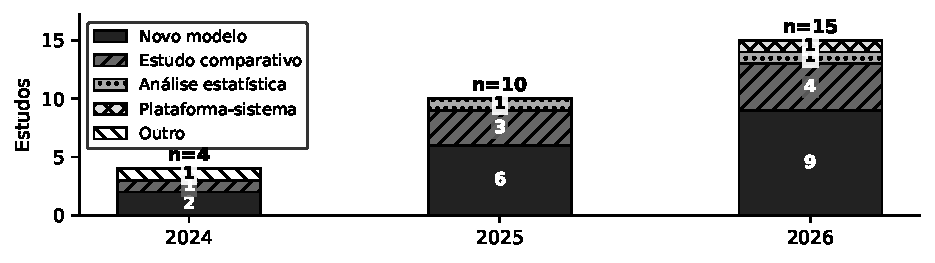
\includegraphics[width=0.78\textwidth]{figuras/fig2_ano_contribuicao.pdf}
\caption{Distribuição dos \nTotal\ estudos por ano e tipo de contribuição.}
\label{fig:ano_contrib}
\end{figure}

\subsection{Tarefas de Classificação e Recortes do Dataset (QP2)}

Pela Tabela~\ref{tab:recorte}, quase toda a literatura usa séries inerciais
(\nModIMU/\nTotal), combinando giroscópio e acelerômetro. O PDNMS e metadados
entram como apoio, salvo dois estudos restritos ao
questionário~\cite{ouabd_parkinsons_2026,padilha_parkinsons_2024}. Entre os
\nModIMU\ trabalhos com IMU, \nTarIMUTodas/\nModIMU\ usam todas as 11 tarefas
motoras, \nTarIMUSubconj/\nModIMU\ apenas um subconjunto e \nPunhoIMUAmbos/\nModIMU\
ambos os punhos, havendo omissões de relato (\nTarIMUNaoRep/\nModIMU\ sem
detalhar tarefas, \nPunhoIMUNaoRep/\nModIMU\ sem especificar punho e
\nSensIMUVazio/\nModIMU\ sem informar sensores~\cite{xing_asa-dsnet_2025}, além de
``IMU de 6 canais'' na categoria Outro~\cite{wei_sgc-rml_2026}, sendo os outros
dois registros sem campo de sensores os estudos sem IMU).

O $N$ amostral consta em \nPartRep/\nTotal\ artigos (\nPartMin--\nPartMax\
participantes, mediana \nPartMediana). Frente ao PADS oficial (276~PD, 79~HC,
114~DD), há divergências em~\cite{djemaa_quantifying_2026} (295/71/103),
\cite{zannat_label-efficient_2026} (291/79/99) e~\cite{vu_simple_2026} (HC=114 e
DD=79 invertidos). Domina PD$\times$HC (\nCenPDHC/\nTotal, \pctCenPDHC),
enquanto PD$\times$DD (\nCenPDDD/\nTotal), 3 classes (classificação simultânea
PD, DD e HC, \nCenTresClasses/\nTotal), DD contra HC (DD$\times$HC,
\nCenDDHC/\nTotal) e outros recortes (Outro, \nCenOutro/\nTotal) aparecem menos.

\begin{table}[htbp]
\centering
\caption{Recorte do dataset PADS nos \nTotal\ estudos (QP2). *Campos multirrótulo (somas acima de 100\%); contagens na ordem das categorias.}
\label{tab:recorte}
{\scriptsize
\setlength{\tabcolsep}{3.5pt}
\begin{tabular}{@{}l l l r@{}}
\toprule
\textbf{Dimensão} & \textbf{Categorias (na ordem das contagens)} & \textbf{Contagens ($n$)} & \textbf{Base} \\
\midrule
Modalidade* & Série temporal (IMU) / Questionário (PDNMS) / Metadados & 27; 9; 8 & $N=29$ \\
Tarefas motoras & Todas / Subconjunto / Não rep. / N/A & 14; 7; 6; 2 & $N=29$ \\
Sensores* & Giroscópio / Acelerômetro / Outro / Não rep. ou N/A & 25; 24; 1; 3 & $N=29$ \\
Punho(s) & Ambos / Não rep. / Esq. ou Dir. (1 cada) / N/A & 16; 9; 2; 2 & $N=29$ \\
Cenários* & PD$\times$HC / PD$\times$DD / 3 classes / Outro / DD$\times$HC / N/A & 20; 15; 7; 5; 2; 1 & $N=29$ \\
\bottomrule
\end{tabular}
}
\end{table}


\subsection{Pré-processamento, Atributos e Modelos (QP3)}

Na entrada dos modelos, predominam séries temporais (categoria ``Série bruta''
do formulário, \nRepBruta/\nTotal, \pctRepBruta) sobre atributos manuais
(\nRepHandcrafted/\nTotal), além do uso pontual de tempo-frequência e
BOSS/\textit{embeddings} (\nRepTF/\nTotal\ cada). Como a categoria ``Série bruta''
reuniu sinais puros e pré-processados, a análise dos \nModIMU\ estudos com IMU
mostra preparos muito distintos: oito removem o transiente vibratório inicial, em regra de 0,5~s como
no artigo-base~\cite{varghese_machine_2024} (e 1~s em um caso). Na filtragem,
cinco corrigem a gravidade por $\ell_1$-\textit{trend filtering} ou pelo
\textit{script} oficial~\cite{padilha_identificacao_2025}, quatro aplicam
filtros passa-faixa ou Butterworth até 20~Hz~\cite{win_checkpd_2026}, dois
decompõem sub-bandas na própria rede e dois declaram não filtrar, havendo ainda
casos pontuais de subtração da média e suavização. Só três reamostram a taxa de
100~Hz (para 64, 40 ou 20~Hz). Quanto à segmentação, cinco dividem séries
longas em blocos de 1.024 pontos e 13 trabalham com sub-janelas curtas
(1--4~s ou 20--512 amostras), por vezes sobrepostas~\cite{gao_coverage-aware_2026}.
Na escala, 12 relatam padronização \textit{z-score} ou por canal (sete restrita
ao treino ou ao sujeito~\cite{djemaa_quantifying_2026} e cinco sem explicitar o
escopo), dois citam normalização genérica e os demais omitem a etapa.

Na modelagem (Figura~\ref{fig:cen_fam}), a família DL lidera (\nFamDL/\nTotal,
\pctFamDL), seguido de ML clássico (\nFamML/\nTotal),
híbridos/\textit{ensemble} (\nFamHybrid), generativos (\nFamGen) e
auto-supervisionados (SSL, \nFamSSL), com foco em PD$\times$HC. No
desbalanceamento, \nBalNenhum/\nTotal\ não aplicam correção, e o restante usa
perturbações ou ponderação (\nBalOutro), SMOTE (\nBalSMOTE) e GANs (\nBalGAN),
com \nBalNaoRep\ sem relato e \nBalNA\ N/A.

\begin{figure}[htb]
\centering
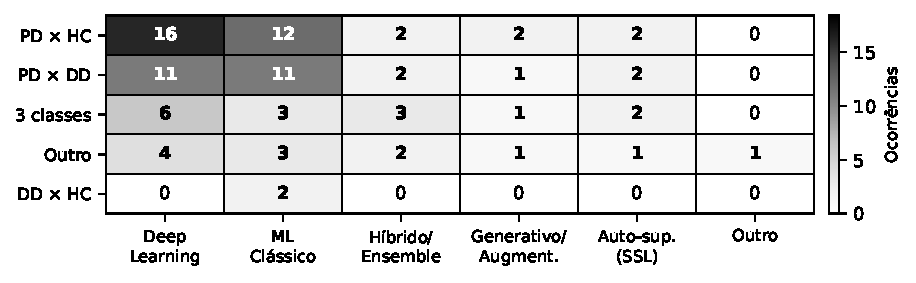
\includegraphics[width=0.78\textwidth]{figuras/fig3_cenario_familia.pdf}
\caption{Cenários de classificação vs.\ famílias de algoritmos ($N=\nTotal$).}
\label{fig:cen_fam}
\end{figure}

\subsection{Validação, Métricas, Vazamento e Desempenho (QP4)}

Pela Tabela~\ref{tab:validacao}, \textit{k-fold} (validação cruzada em $k$ dobras,
\nValKfold/\nTotal) predomina, com \textit{hold-out} (partição fixa treino/teste,
\nValHoldout), enquanto CV aninhada (\nValAninhada) e LOSO
(\textit{leave-one-subject-out}, \nValLOSO~\cite{sridhar_early_2026}) são raras.
Embora \nUnidPart/\nAplicaveisVaz\ (\pctUnidPart) preditivos dividam por
participante (6 inferidos, 5 sem relato), a Figura~\ref{fig:risco_vaz} mostra
que só \nRiscoBaixo/\nAplicaveisVaz\ (\pctRiscoBaixoAplic) mantêm risco baixo de
vazamento (Seção~\ref{sec:desvio_qa}). Outros \nRiscoModerado\ têm risco de
vazamento moderado (pré-processamento omitido) e \nRiscoAlto, alto, por
balanceamento ou janelamento pré-\textit{split}~%
\cite{zannat_label-efficient_2026,abioye_improving_2025,wang_parkinsons_2025,yu_improved_2024}.

\begin{table}[htbp]
\centering
\caption{Protocolos de validação e risco de vazamento reportado (QP4). *Multirrótulo; $N=27$ exclui \nNaoAplicaveisVaz\ análises estatísticas (N/A).}
\label{tab:validacao}
{\scriptsize
\setlength{\tabcolsep}{3.2pt}
\begin{tabular}{@{}l l l r@{}}
\toprule
\textbf{Aspecto} & \textbf{Categorias (na ordem das contagens)} & \textbf{Contagens ($n$)} & \textbf{Denominador} \\
\midrule
Estratégia* & k-fold CV / Hold-out / CV aninhada / Não rep. / LOSO / Outra & 24; 9; 6; 3; 1; 1 & $N=29$ \\
Unid. particionamento & Participante / Não reportado / Não se aplica & 22 (81,5\%); 5; 2 & $N=27$ (+2 N/A) \\
Separação participante & Sim explícita / Sim inferida / Pouco claro / N/A & 16; 6; 5; 2 & $N=27$ (+2 N/A) \\
Momento balanceam. & Só no treino / Antes do split / Não rep. / N/A & 11; 4; 2; 12 & $N=29$ \\
Pré-proc. só no treino & Sim / Não / Não reportado / Não se aplica & 10; 4; 13; 2 & $N=27$ (+2 N/A) \\
Risco de vazamento & Baixo / Moderado / Alto / Indeterminado / N/A & 10; 11; 4; 2; 2 & $N=27$ (+2 N/A) \\
\bottomrule
\end{tabular}
}
\end{table}


Nenhum estudo fez validação externa entre bases (\nValExtSim/\nTotal): embora
\nMultiBase\ combinem bases e~\cite{abioye_improving_2025} cite o PADS para
generalização, todos retreinaram internamente. Nas métricas, F1
(\nMetFOne/\nTotal) e acurácia (\nMetAcc/\nTotal) superam Bal.\ Acc.\
(\nMetBalAcc/\nTotal) e AUC (\nMetAUC/\nTotal). A Tabela~\ref{tab:desempenho}
lista o melhor resultado por \texttt{row\_id}, sem comparação direta.

\begin{figure}[htb]
\centering
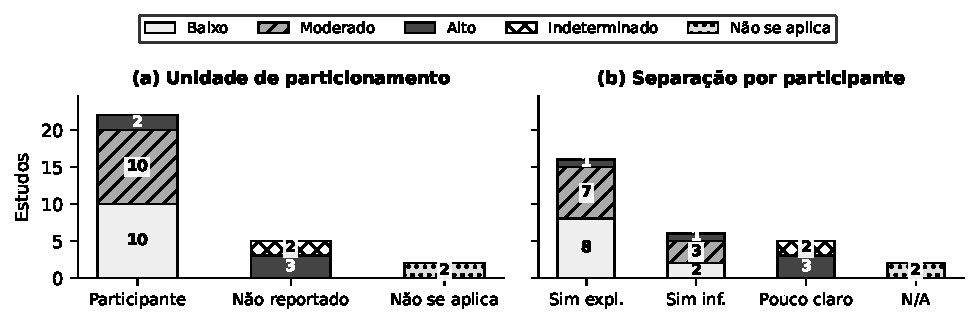
\includegraphics[width=0.78\textwidth]{figuras/fig4_risco_vazamento.pdf}
\caption{Risco de vazamento por unidade (a) e separação por sujeito (b).}
\label{fig:risco_vaz}
\end{figure}

\begin{table}[htbp]
\centering
\caption{Melhor resultado (\texttt{row\_id}, sem ranqueamento). HO = \textit{hold-out}, Anin.\ = CV aninhada, LOTO = \textit{leave-one-task-out}, Vaz.\ = risco de vazamento.}
\label{tab:desempenho}
{\tiny
\setlength{\tabcolsep}{1.4pt}
\renewcommand{\arraystretch}{0.68}
\begin{tabular*}{0.99\textwidth}{@{}r@{\extracolsep{\fill}} >{\raggedright\arraybackslash}p{3.10cm} >{\raggedright\arraybackslash}p{2.12cm} >{\raggedright\arraybackslash}p{2.52cm} >{\raggedright\arraybackslash}p{1.12cm} >{\raggedright\arraybackslash}p{2.36cm} l@{}}
\toprule
\textbf{ID} & \textbf{Estudo} & \textbf{Cenário} & \textbf{Modelo/Método} & \textbf{Métrica} & \textbf{Resultado} & \textbf{Validação (Vaz.)} \\
\midrule
2 & \cite{djemaa_quantifying_2026} & Outro (PD vs. non-PD) & BTE+SMOTE+RF & AUC & 0,842 $\pm$ 0,043 & k-fold (Baixo) \\
13 & \cite{mohtavipour_deep_2026} & PD$\times$HC & Multi-stream CNN-Transf. & Bal. Acc. & 85,89\% $\pm$ 3,93\% & k-fold (Mod.) \\
21 & \cite{sridhar_early_2026} & PD$\times$HC & CNN-BiLSTM + Attention & Accuracy & 95,30\% $\pm$ 1,10\% (10-fold) & Anin.+LOSO+k-fold (Baixo) \\
23 & \cite{zannat_label-efficient_2026} & PD$\times$HC & Interleaved self-attn (ours) & AUROC & 0,963 & LOTO+k-fold (Alto) \\
32 & \cite{huang_self-supervised_2025} & Outro (PL vs. PD) & Ours & Acc/F1/AUC & 81,00\% / 0,81 / 0,81 & HO (Mod.) \\
40 & \cite{zhang_generative_2025} & PD$\times$HC & BOSS+SVM (TremorGANs) & Accuracy & 87,60\% $\pm$ 1,40\% & k-fold (Baixo) \\
44 & \cite{gao_coverage-aware_2026} & PD$\times$HC & RBF-SVM (Ours) & Bal. Acc. & 80,52\% $\pm$ 9,08\% & Anin.+k-fold (Baixo) \\
47 & \cite{abioye_improving_2025} & 3 classes & Stacking (CatBoost+RF+LR) & Accuracy & 100,00\% & HO+k-fold (Alto) \\
49 & \cite{abola_differentiating_2025} & Outro (6 grupos) & Reg. Logística Multinom. & Pseudo R$^2$ & 0,068 (LR $\chi$$^2$=1740, p<0,001) & Não rep. (N/A) \\
51 & \cite{xu_adaptive_2024} & PD$\times$DD (StretchHold) & ADAMIL (Ours) & Accuracy & 81,44\% & k-fold (Mod.) \\
54 & \cite{ren_baseline_2026} & N/A (Correl.) & Correl. de Spearman & Spearman r & r = -0,171 (p=0,0071) & Não rep. (N/A) \\
70 & \cite{varghese_machine_2024} & PD$\times$HC & Stacking (IMU+PDNMS) & Bal. Acc. & 91,16\% (4,92\%) & Anin.+k-fold (Baixo) \\
76 & \cite{xing_asa-dsnet_2025} & 3 classes & ASA-DSNet & Accuracy & 80,85\% & Anin.+k-fold (Indet.) \\
77 & \cite{pathirathna_neurolens_2026} & PD$\times$HC & 1D CNN (8-bit) & Bal. Acc. & 70,20\% & HO+k-fold (Mod.) \\
79 & \cite{zeebaree_three-class_2027} & 3 classes & Soft-voting XGB-LGBM & Accuracy & 72,28\% $\pm$ 3,19\% & HO+k-fold (Baixo) \\
80 & \cite{zhao_multi-scale_2025} & PD$\times$DD (CrossArms) & MFAM & Accuracy & 81,29\% & k-fold (Mod.) \\
81 & \cite{vasisht_energy_2026} & PD$\times$HC & Random Forest & Accuracy & 82,86\% & HO+k-fold (Mod.) \\
83 & \cite{kalathoti_blockchain-enabled_2026} & Outro (PD vs. No PD) & CNN-Transformer & Accuracy & 97,29\% & k-fold (Mod.) \\
85 & \cite{suk-ieam_smartwatch-based_2025} & PD$\times$HC & 1D CNN (Finger-to-Finger) & Accuracy & 87,32\% & Não rep. (Indet.) \\
87 & \cite{wang_parkinsons_2025} & PD$\times$HC & MSF-CANet & Accuracy & 92,39\% & Anin.+k-fold (Alto) \\
89 & \cite{ouabd_parkinsons_2026} & PD$\times$HC & Random Forest & Bal. Acc. & 93,24\% & HO+k-fold (Baixo) \\
90 & \cite{vu_simple_2026} & PD$\times$HC & LR & Bal. Acc. & 79,26\% $\pm$ 5,50\% & Anin.+k-fold (Baixo) \\
92 & \cite{yu_improved_2024} & PD$\times$HC & CA\_LSTM\_FCN (acc + rot) & Accuracy & 92,15\% & k-fold (Alto) \\
99 & \cite{win_checkpd_2026} & PD$\times$HC (Relaxed/Rest) & Conv1D-BiLSTM & ROC AUC & 0,842 & HO+k-fold (Baixo) \\
101 & \cite{wei_sgc-rml_2026} & 3 classes & PatchTST + Quality & AUC & 0,825 & HO+k-fold (Baixo) \\
104 & \cite{haque_eco-xpd_2026} & PD$\times$HC & Eco-xPD (c/ xReDA) & F1-score & 93,60\% $\pm$ 1,03\% & HO (Mod.) \\
105 & \cite{padilha_identificacao_2025} & PD$\times$HC (DP vs. CO) & LightGBM & Accuracy & 84,05\% $\pm$ 3,16\% & k-fold (Mod.) \\
108 & \cite{padilha_parkinsons_2024} & PD$\times$HC & Random Forest & Bal. Acc. & 87,00\% & k-fold (Mod.) \\
109 & \cite{lobo_parkinsons_2025} & DD$\times$HC & Extra Trees & Bal. Acc. & 82,48\% & k-fold (Mod.) \\
\bottomrule
\end{tabular*}
}
\end{table}


\subsection{Qualidade e Reprodutibilidade (QP4)}

Qualidade metodológica média (QA): \qaMediaPct\ (mediana \qaMedianaPct,
\qaMinPct--\qaMaxPct), com \nQAMedia/\nTotal\ na faixa Média, \nQAAlta\ Alta e
\nQABaixa\ Baixa (Seção~\ref{sec:desvio_qa}). Na Figura~\ref{fig:qa}, QA1--QA2
vão bem, mas falham QA4 (parcial: \nQAQuatroPart/\nTotal) e QA5:
\nCodDisponivel/\nTotal\ (\pctCodDisponivel) abrem
código~\cite{mohtavipour_deep_2026,xu_adaptive_2024,wei_sgc-rml_2026} ou
ambos~\cite{varghese_machine_2024}.

\begin{figure}[htb]
\centering
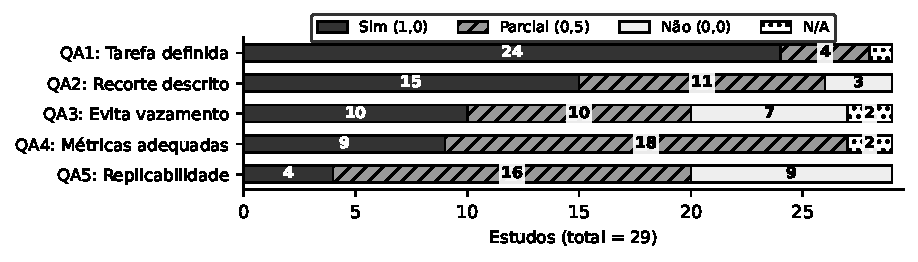
\includegraphics[width=0.78\textwidth]{figuras/fig5_qa.pdf}
\caption{Distribuição das respostas de qualidade (QA1--QA5) nos \nTotal\ estudos.}
\label{fig:qa}
\end{figure}

\subsection{Lacunas Identificadas e Oportunidades (QP5)}

A Tabela~\ref{tab:lacunas} sintetiza cinco lacunas (\nSemLimitacao\ sem limitações
e \nSemLacuna\ sem trabalhos futuros): multimodalidade/explicabilidade
(XAI)/calibração (\nLacunaMultimodalXAI/\nTotal), severidade/vida livre
(\nLacunaLongitSev/\nTotal), coortes externas (\nLacunaValExt/\nTotal) e
diagnóstico diferencial (\nLacunaPDDD/\nTotal), com \pctCodNenhum\ sem
código/dados e \pctCodNaoRep\ sem menção.

\begin{table}[htbp]
\centering
\caption{Síntese temática das limitações reportadas, lacunas e reprodutibilidade nos \nTotal\ estudos (QP5).}
\label{tab:lacunas}
{\scriptsize
\setlength{\tabcolsep}{3pt}
\begin{tabular}{@{}>{\raggedright\arraybackslash}p{3.8cm} r >{\raggedright\arraybackslash}p{4.0cm} >{\raggedright\arraybackslash}p{4.1cm}@{}}
\toprule
\textbf{Tema / Lacuna} & \textbf{$n/N$ (\%)} & \textbf{Exemplos no corpus} & \textbf{Implicação para o PADS} \\
\midrule
Ausência de validação externa / coortes multicêntricas & 15/29 (51,7\%) & \cite{djemaa_quantifying_2026}, \cite{zannat_label-efficient_2026}, \cite{huang_self-supervised_2025} (e outros 12) & Treino/teste restrito ao PADS; validação externa = 0/29. \\
Dificuldade no diagnóstico diferencial (PD$\times$DD) & 11/29 (37,9\%) & \cite{zannat_label-efficient_2026}, \cite{huang_self-supervised_2025}, \cite{zhang_generative_2025} (e outros 8) & Menor acurácia na fronteira PD vs.\ DD/tremor essencial. \\
Falta de severidade clínica (MDS-UPDRS/H\&Y) e vida livre/longitudinal & 17/29 (58,6\%) & \cite{zannat_label-efficient_2026}, \cite{huang_self-supervised_2025}, \cite{abola_differentiating_2025} (e outros 14) & Falta MDS-UPDRS/H\&Y e coleta em vida livre. \\
Falta de multimodalidade, XAI, calibração e justiça demográfica & 20/29 (69,0\%) & \cite{djemaa_quantifying_2026}, \cite{zhang_generative_2025}, \cite{abioye_improving_2025} (e outros 17) & Fusão, explicabilidade clínica, calibração e controle de vazamento. \\
Indisponibilidade de código/dados derivados (reprodutibilidade) & 25/29 (86,2\%) & \cite{djemaa_quantifying_2026}, \cite{zannat_label-efficient_2026}, \cite{huang_self-supervised_2025} (e outros 22) & Compartilhamento de código/dados em apenas \nCodDisponivel/\nTotal. \\
\bottomrule
\end{tabular}
}
\end{table}


\subsection{Literatura Cinzenta: Preprints e Análise de Sensibilidade}
\label{sec:preprints}

Os \nPreprints\ \textit{preprints} (2026, DL, Tabela~\ref{tab:preprints}) focam
PD$\times$HC (só 1 em PD$\times$DD), com QA média maior (\qaMediaPrePct\
vs.\ \qaMediaRevPct) e mais risco baixo de vazamento pelo controle no
\textit{augmentation}~\cite{djemaa_quantifying_2026}, salvo risco alto de
vazamento por janelamento~\cite{zannat_label-efficient_2026}. Sem eles
($n=\nRevisadosPares$), 2026 cai (\pctAnoDoisSeis\ a \pctRevAnoDoisSeis,
\nRevAnoDoisSeis/\nRevisadosPares), risco baixo de vazamento (\pctRiscoBaixoAplic\
a \pctRevRiscoBaixoAplic) e código (\pctCodDisponivel\ a \pctRevCodDisp),
mantendo DL, PD$\times$HC (PD$\times$DD: \pctRevPDDD\ vs.\ \pctCenPDDD) e
\nValExtSim/\nRevisadosPares\ em validação externa.

\begin{table}[htbp]
\centering
\caption{Revisados ($n=23$) vs.\ \textit{preprints} ($n=6$) e sensibilidade total ($n=29$).}
\label{tab:preprints}
{\scriptsize
\setlength{\tabcolsep}{3.5pt}
\renewcommand{\arraystretch}{0.74}
\begin{tabular*}{0.78\textwidth}{@{}l@{\extracolsep{\fill}} r r r@{}}
\toprule
\textbf{Indicador} & \textbf{Revisados ($n=23$)} & \textbf{Preprints ($n=6$)} & \textbf{Total ($n=29$)} \\
\midrule
Publicação em 2026 & 9/23 (39,1\%) & 6/6 (100,0\%) & 15/29 (51,7\%) \\
Contribuição: Novo modelo & 13/23 & 4/6 & 17/29 \\
Cenário PD$\times$DD & 14/23 (60,9\%) & 1/6 (16,7\%) & 15/29 (51,7\%) \\
Família: Deep Learning & 16/23 (69,6\%) & 6/6 (100,0\%) & 22/29 (75,9\%) \\
Separação por participante (Sim) & 16/21 & 6/6 & 22/27 \\
Risco de vazamento Baixo & 6/21 (28,6\%) & 4/6 (66,7\%) & 10/27 (37,0\%) \\
Qualidade QA (faixa Alta) & 5/23 (21,7\%) & 4/6 (66,7\%) & 9/29 (31,0\%) \\
Qualidade QA (média) & 60,6\% & 80,0\% & 64,6\% \\
Código/dados disponíveis & 2/23 & 2/6 & 4/29 \\
\bottomrule
\end{tabular*}
}
\end{table}


\section{Discussão} \label{sec:discussao}

\subsection{Achados Principais, Estudo-Base e Recomendações}

Nos estudos avaliados, há contraste claro entre modelos avançados e rigor:
\nFamDL/\nTotal\ (\pctFamDL) usam \textit{deep learning}, mas só
\nRiscoBaixo/\nAplicaveisVaz\ (\pctRiscoBaixoAplic) mantêm risco baixo de
vazamento. O artigo-base~\cite{varghese_machine_2024} adotou CV aninhada,
acurácia balanceada, código público e PD$\times$DD, mas poucos mantiveram esses
critérios (\nValAninhada/\nTotal, \nMetBalAcc/\nTotal\ e
\nCodDisponivel/\nTotal, nessa ordem). Protocolos sem controle ou com
balanceamento pré-\textit{split}~%
\cite{abioye_improving_2025,wang_parkinsons_2025,yu_improved_2024} chegam a
92\%--100\%, incomparáveis à divisão por
sujeito~\cite{zeebaree_three-class_2027,vu_simple_2026}, conforme alertam
revisões~\cite{pinto_neto_machine_2026,ouabd_overview_2026}.

Para avançar a área, quatro cuidados são prioritários: separar por participante
antes de janelar, normalizar ou gerar amostras; usar métricas balanceadas
(Bal.\ Acc., F1-macro, MCC) e calibração; focar tarefas com DD; e abrir código,
lendo \textit{preprints} (\nPreprints) com cautela.

\subsection{Ameaças à Validade}

Na busca (I7), focar citações ao artigo-base~\cite{varghese_machine_2024} pode
omitir quem cita só o
PhysioNet~\cite{PhysioNet-parkinsons-disease-smartwatch-1.0.0}, além de faltarem
corte e rejeições. Na extração (I2), IA sem dupla revisão nem $\kappa$ deixa
\nPontosRevisao\ pontos e metadados pendentes. Os \textit{preprints} (B4) foram
tratados na Seção~\ref{sec:preprints}; QA e vazamento (I4, I5) avaliam relato, e
a validação externa (I1) requer revisão em \nMultiBase/\nTotal\ multibase
e~\cite{abioye_improving_2025}.

\section{Conclusão} \label{sec:conclusao}

Nos \nTotal\ estudos com PADS (\nRevisadosPares\ revisados e \nPreprints\
\textit{preprints}), predominam \textit{deep learning} (\nFamDL/\nTotal) e
PD$\times$HC (\nCenPDHC/\nTotal). Só \nRiscoBaixo/\nAplicaveisVaz\
(\pctRiscoBaixoAplic) aplicáveis têm risco baixo, nenhum tem validação externa
(\nValExtSim/\nTotal) e só \nCodDisponivel/\nTotal\ (\pctCodDisponivel) abrem
código/dados --- padrão mantido sem \textit{preprints}. Avançar exige divisão
por sujeito, foco em DD, código aberto e, em extensões do protocolo, campos de
pré-processamento (filtragem, corte inicial, janela e escopo de escala). A
planilha de extração não será disponibilizada externamente, ficando apenas
sintetizada aqui.


\bibliographystyle{sbc}
\bibliography{referencias}

\end{document}
